% Figure 4 — response of the event signal a = s*nu*mu (standalone, vector PDF).
\documentclass[border=3pt]{standalone}
\usepackage{amsmath}
\usepackage{tikz}
\usepackage{pgfplots}
\pgfplotsset{compat=1.17}
\begin{document}
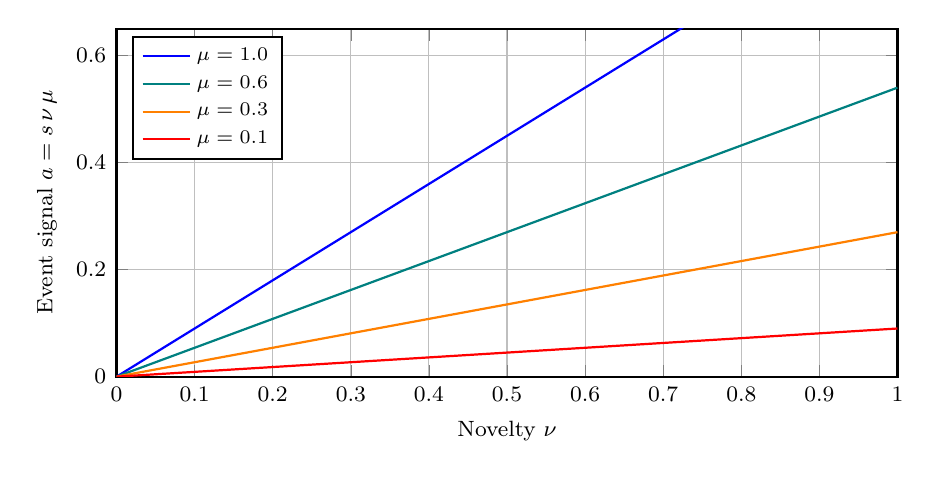
\begin{tikzpicture}
\begin{axis}[
  width=11.5cm, height=6.0cm, font=\footnotesize,
  xlabel={Novelty $\nu$}, ylabel={Event signal $a=s\,\nu\,\mu$},
  xmin=0,xmax=1,ymin=0,ymax=0.65, domain=0:1, samples=60,
  legend style={at={(0.02,0.98)},anchor=north west,font=\scriptsize},
  ymajorgrids, xmajorgrids, thick
]
\addplot[blue,thick]   {0.9*x*1.0};
\addplot[teal,thick]   {0.9*x*0.6};
\addplot[orange,thick] {0.9*x*0.3};
\addplot[red,thick]    {0.9*x*0.1};
\legend{$\mu=1.0$,$\mu=0.6$,$\mu=0.3$,$\mu=0.1$}
\end{axis}
\end{tikzpicture}
\end{document}
